We now wish to fit a time series model to the data described in Section \ref{data}.
As can be seen from Figure \ref{tweets_plot}, there are seasonal and trend components
present in the underlying data set and what also appears to be non-constant variance.

Thus, we will need to apply transformations to the time series in order to determine
the underlying time series model.

\begin{subsection}{Transformations}\label{transformations}
  Let $\{X_t\}$ for $t=1,2,\dots, 144$ denote the observations
  of the time series described in Section \ref{data}. To remove the non-constant variance
  we apply the Box-Cox transformation $\log$ to the observations $\{X_t\}$ to arrive
  at the mean-corrected data $Y_t = \log(X_t) - E(\log(X_t))$ for $t=1,2,\dots, 144$.
  As can be seen from Figure \ref{log_plot}, this transformation has made the variance
  of the data constant.

  \begin{figure}[!h]
    \centerline{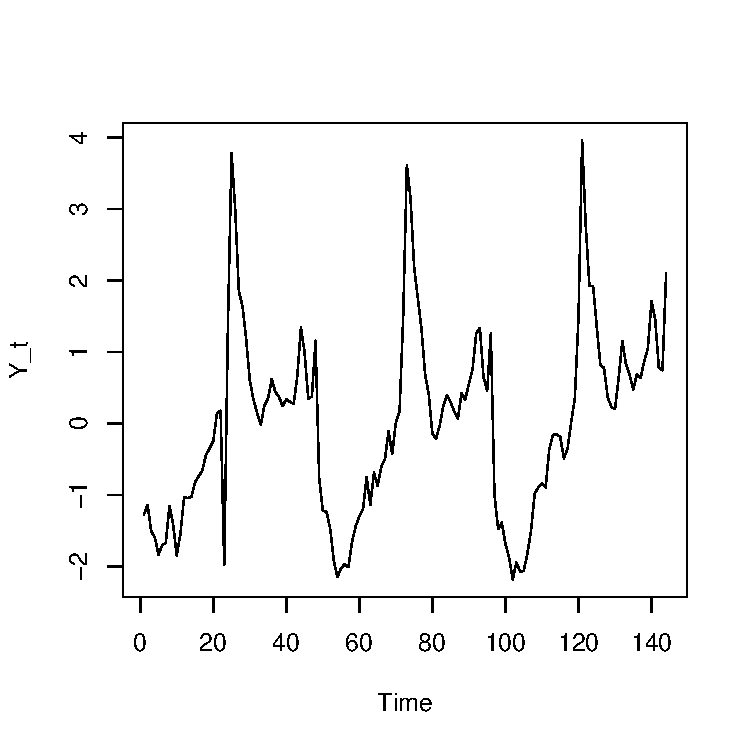
\includegraphics[scale=0.75]{../analysis/plots/log_plot}}
    \caption{Plot of Box-Cox transformed data $Y_t = \log(X_t) - E(\log(X_t))$.}\label{log_plot}
  \end{figure}

  The seasonality and trend noticed with the untransformed data is still present in
  the transformed data. Through differencing, we hope to characterize the underlying
  seasonality and trend of the data.

  Knowing that the observations come from data with a period of 48 hours, it makes sense
  to remove the seasonality by applying the differencing operator $\left(1 - B^{48}\right)$ to $Y_t$.
  Applying this transformation results in Figure \ref{seasonal_plot}.

  \begin{figure}[!h]
    \centerline{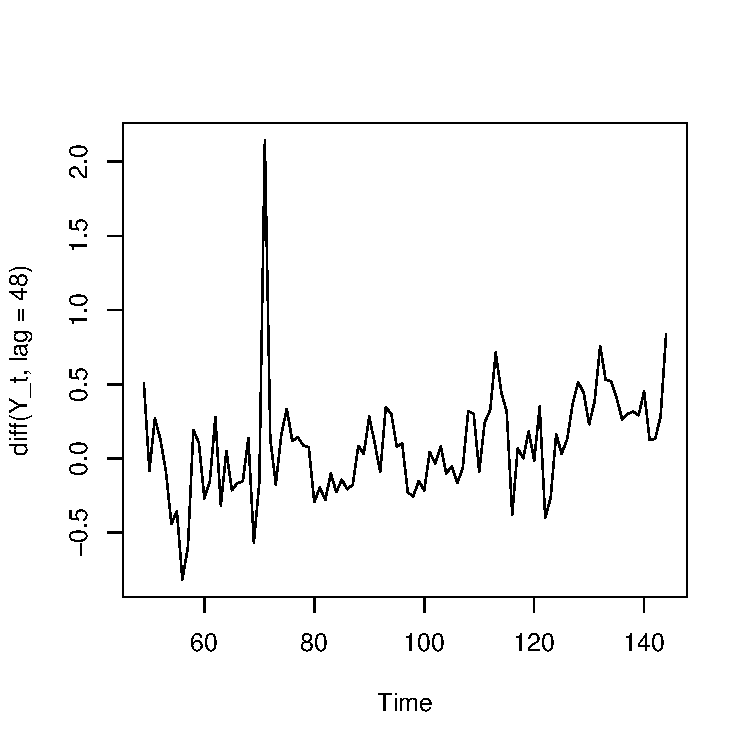
\includegraphics[scale=0.75]{../analysis/plots/seasonal_plot}}
    \caption{Plot of data $\left(1 - B^{48}\right)Y_t$.}\label{seasonal_plot}
  \end{figure}

  As can be seen from the figure, the seasonality has been removed. The plots
  of the ACF and the PACF of $\left(1 - B^{48}\right)Y_t$ are found in Figure \ref{cf_seasonal}.

  \begin{figure}[!h]
    \begin{subfigure}[b]{.48\textwidth}
      \centering
      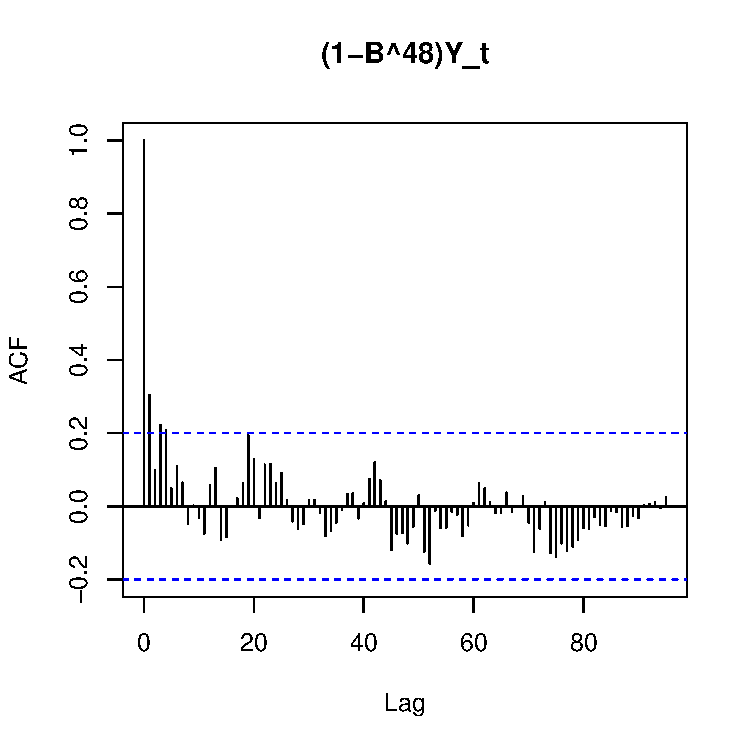
\includegraphics[scale=0.5]{../analysis/plots/seasonal_acf}
    \end{subfigure}
    \begin{subfigure}[b]{.48\textwidth}
      \centering
      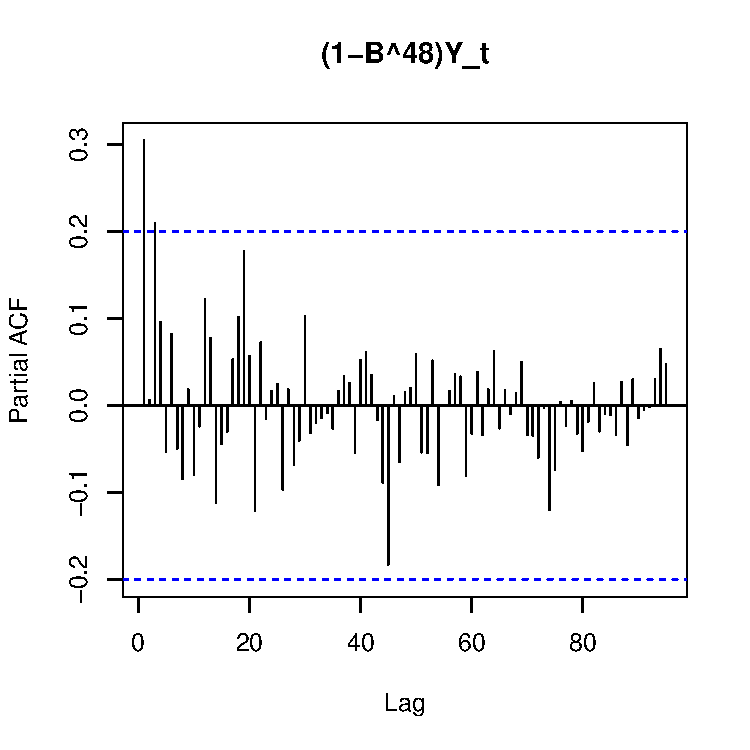
\includegraphics[scale=0.5]{../analysis/plots/seasonal_pacf}
    \end{subfigure}
    \caption{ACF and PACF of $\left(1 - B^{48}\right)Y_t$.}\label{cf_seasonal}
  \end{figure}

  These plots suggest that a seasonal AR model of order 1 or 3 may be
  appropriate as the ACF slowly decreases to 0 while the PACF stops abruptly
  after lag 3.

  However, as can also be seen in Figure \ref{seasonal_plot}, there is still a
  trend component present. This trend appears linear suggesting that applying
  the difference operator $(1 - B)$ to $\left(1 - B^{48}\right)Y_t$ will remove
  this trend. The results of applying the operator are found in Figure \ref{trend_plot}.

  \begin{figure}[!h]
    \centerline{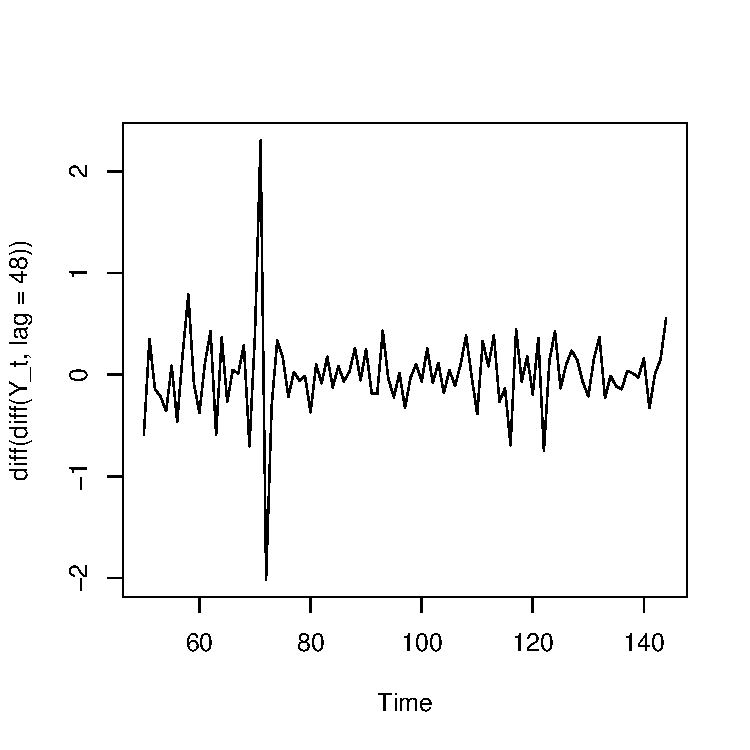
\includegraphics[scale=0.75]{../analysis/plots/trend_plot}}
    \caption{Plot of data $(1-B)\left(1 - B^{48}\right)Y_t$.}\label{trend_plot}
  \end{figure}

  The plot in Figure \ref{trend_plot} shows that the trend component.
  The plots of the ACF and the PACF of
  $(1-B)\left(1 - B^{48}\right)Y_t$ are found in Figure \ref{cf_trend}.

  \begin{figure}[!h]
    \begin{subfigure}[b]{.48\textwidth}
      \centering
      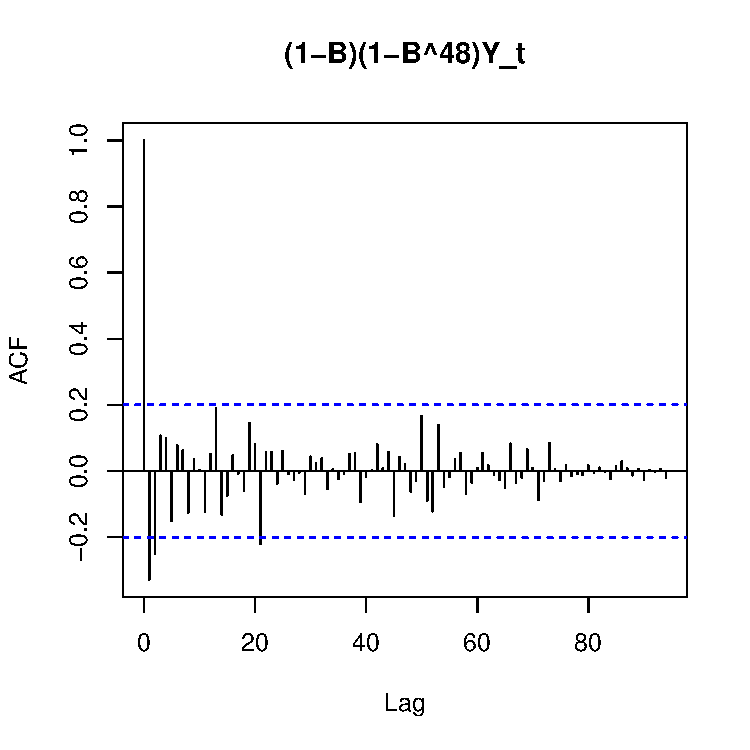
\includegraphics[scale=0.5]{../analysis/plots/trend_acf}
    \end{subfigure}
    \begin{subfigure}[b]{.48\textwidth}
      \centering
      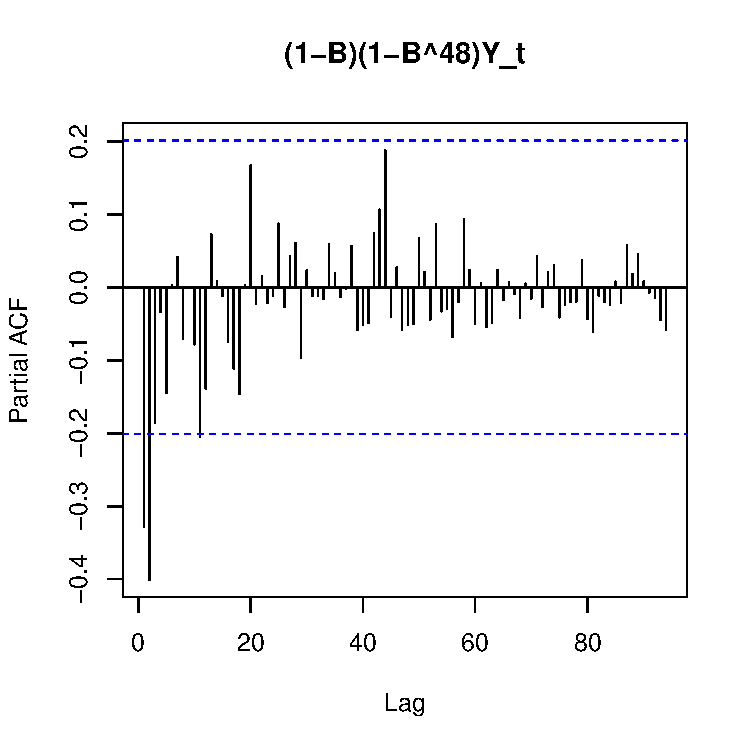
\includegraphics[scale=0.5]{../analysis/plots/trend_pacf}
    \end{subfigure}
    \caption{ACF and PACF of $(1-B)\left(1 - B^{48}\right)Y_t$.}\label{cf_trend}
  \end{figure}

  These plots suggest a possible AR model of order 2 for the trend component as the ACF
  slowly decreases to
  0 while the PACF stops abruptly after lag 2. It is also possible for an MA component
  to be present so we will investigate models of the form ARMA($p$, $q$) for $p,q=1,2$
  for the trend component.
\end{subsection}

\begin{subsection}{Model Selection}
  The findings from Section \ref{transformations} suggest fitting the data $\{Y_t\}$
  to a seasonal ARIMA model. Specifically, a model of the form
  \[
    \text{SARIMA}(p, 1, q)\times (P, 1, 0)_{48}
  \]
  where $p, q \in \{0, 1, 2\}$ and $P \in \{1, 3\}$.

  Using the programming language R, we examine the AIC statistic associated to
  each of the different possible models suggested and choose the model that
  minimizes this statistic. Due to the limitations of the available hardware,
  we were unable to fit SARIMA models to the data in which $P=3$ for such a large period.
  Thus, we present the results of testing for $P=1$ alone.

  \begin{table}[h!]
    \centering
    \def\arraystretch{1.25}
    \begin{tabular}{| p{1.5cm} | p{1.5cm} | p{2cm} |}
      \hline
      $p$ & $q$ & AIC \\
      \hline
      0 & 1 & 77.00203 \\
      0 & 2 & 75.06627 \\
      1 & 0 & 99.46614 \\
      1 & 1 & \texttt{NaN} \\
      1 & 2 & 78.04194 \\
      2 & 0 & 85.23537 \\
      2 & 1 & 77.33328 \\
      2 & 2 & 78.92953 \\
      \hline
    \end{tabular}
    \vspace{3mm}
    \caption{AIC values for different possible SARIMA$(p,1,q)\times(1,1,0)_{48}$
      models fitted to the data $Y_t = \log(X_t) - E(\log(X_t))$.}\label{aic_table}
  \end{table}

  Note that hardware limitations also prevented us from fitting a model of the
  form $\text{SARIMA}(1,1,1)\times(1,1,0)_{48}$
  to the data so that has been omitted from consideration as well. Table \ref{aic_table} suggests
  that, if we are to select a model based on minimizing the AIC statistic,
  we should choose to fit the data to a SARIMA$(0,1,2)\times(1,1,0)_{48}$ model.

  Doing so produces the following output in R:
  \begin{lstlisting}[language=R]
Coefficients:
          ma1      ma2     sar1
      -0.6768  -0.2257  -0.1586
s.e.   0.1097   0.1100   0.1441

sigma^2 estimated as 0.1152:  log likelihood = -33.53,  aic = 75.07
  \end{lstlisting}
  The above gives the associated p-values for the coefficients of the model:
  \begin{lstlisting}[language=R]
      ma1          ma2         sar1
6.878613e-10 4.021464e-02 2.709825e-01
  \end{lstlisting}
  Using a significance level of $\alpha=0.05$ suggests that the SAR(1) coefficient
  is not significant. However, removing the seasonal component and fitting the model
  to an MA(2) model results in a worse fit. Thus, we elect to keep the seasonal
  component in the model.

  Thus we fit, our data $Y_t = \log(X_t) - E(\log(X_t))$ to the model
  \begin{align}\label{sarima_model}
    Y_t = \Phi_1Y_{t-48} + Z_t + \theta_1Z_{t-1} + \theta_2Z_{t-2} \quad Z_t \sim \text{WN}(0, \sigma^2) \notag\\
    \Phi_1 = -0.1586, \quad \theta_1 = -0.6768, \quad \theta_2 = -0.2257, \quad \sigma^2 = 0.1152
  \end{align}
  We verify that these residuals are indeed
  a white noise process by examining the plot of their ACF in Figure \ref{res_acf}

  \begin{figure}[!h]
    \centerline{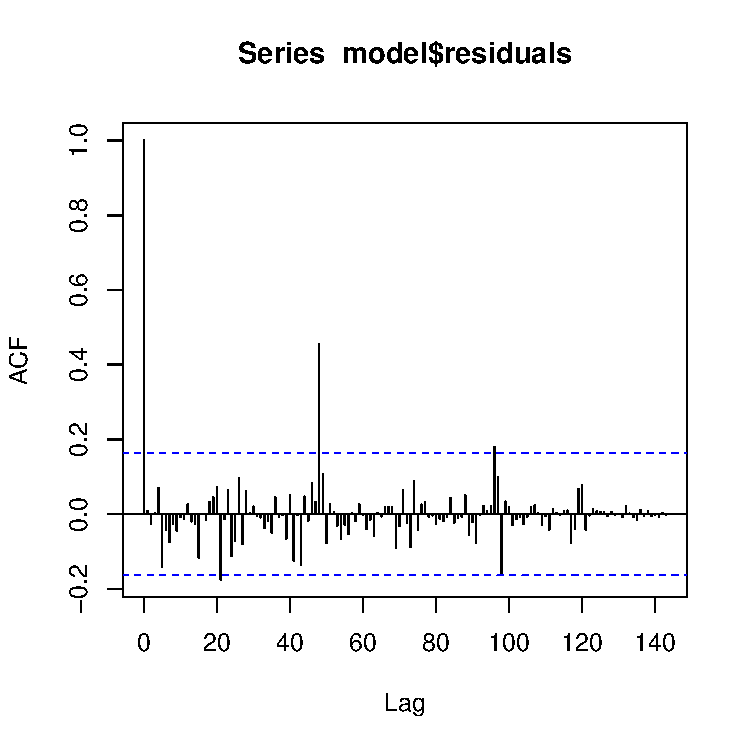
\includegraphics[scale=0.75]{../analysis/plots/res_acf}}
    \caption{Plot of ACF of $Z_t$ in \eqref{sarima_model}.}\label{res_acf}
  \end{figure}

  As almost all of the values fall within the 0-bound, we conclude that this
  process is most likely a white noise process.

\end{subsection}